\section{The Canonical Ensemble and the Partition function}
By repeating the calculation with the last condition which defines the canonical ensemble, i.e. an ensemble where the energy is not fixed and can change while its average $<H>$ remains fixed, we can find $\rho \propto e^{-\beta H}$, where $\beta$ is the Lagrange multiplier correspondent to this latter condition. This can be easily normalized by introducing the \textbf{partition function $\mathcal{Z}$}:
\begin{equation}
    \mathcal{Z}=\int d\Gamma e^{-\beta H}
\end{equation}
which is also known as the \textit{generating function} since it can be used to produce the moments of the distribution and many other quantities.Then our density over the canonical ensemble can be written as:
\begin{equation}
    \rho=\frac{e^{-\beta H}}{\mathcal{Z}}.
\end{equation}
\paragraph*{Internal energy}
Let's look at how we can use the partition function in order to find an expression for $U=<H>$, which corresponds to the \textit{internal energy} of the system in the canonical ensemble:
\begin{equation}
\begin{split}
    U=<H> & =\int d\Gamma\, \frac{e^{-\beta H}}{\mathcal{Z}}\cdot H \\
    & = -\frac{\partial}{\partial \beta}\left[\ln{\int d\Gamma e^{- \beta H}}\right] \\
    & = -\frac{\partial}{\partial \beta}\ln{\mathcal{Z}}.
\end{split}
\end{equation}

For an example, consider the hamiltonian: $H=\sum_i \frac{p_i^2}{2m}$, i.e. an ideal gas composed of N non interacting particles. The partition function of this system is given by:
\begin{equation*}
    \mathcal{Z}=\int d^{3N}q \int d^{3N}p\,e^{-\beta \sum i \frac{p_i^2}{2m}}=V^N \left(\int dp\, e^{-\beta \frac{p^2}{2m}}\right)^{3N}
\end{equation*}
where we used the fact that the hamiltonian do not depend on the position (so the integral over the coordinates for each particle just give us the complete volume $V$ of the system ) and that the momenta are separable into their product. We remain with a gaussian integral, so that we get:
\begin{equation}
    \mathcal{Z}=V^N \left(\frac{2\pi m}{\beta} \right)^{\frac{3N}{2}}
\end{equation}
\begin{equation}
    \implies \ln{\mathcal{Z}}=N\ln{\left[V\left(\frac{2\pi m}{\beta} \right)^{\frac{3}{2}}\right]}
\end{equation}
which we can use to finally find the internal energy:
\begin{equation}
    U= -\frac{\partial}{\partial \beta}\ln{\mathcal{Z}}=N\frac{3}{2\beta}.
\end{equation}
At this point we couldn't go any further; However, we can consider the expression $U=\frac{3}{2}N k_B T$ as a phenomenological knowledge based on experiments, in order to implement this information in our theory. By comparing the two expression, we can easily find that:
\begin{equation}
    \beta=\frac{1}{k_B T}
\end{equation}
and by using instead $U=\frac{3}{2}n R T=\frac{3}{2}N\frac{R}{N_A} T$ we get:
\begin{equation}
    R=N_A \cdot k_B
\end{equation}
which gives us a physical interpretation (and definition) for $\beta$ as well as a relation between $R, N_A$ and $k_B$.
\paragraph*{Heat capacity}
Another quantity which we wish to extract is $\frac{\partial^2}{\partial \beta^2}\ln{\mathcal{Z}}=-\frac{\partial U}{\partial \beta}$:
\begin{equation*}
\begin{split}
    -\frac{\partial U}{\partial\beta} & = -\frac{\partial}{\partial\beta}\left[\frac{\int d\Gamma\, e^{-\beta H}\cdot H}{\int d\Gamma\, e^{-\beta H}}\right] \\
    & =\frac{\int d\Gamma\, H^2 e^{-\beta H}}{\int d\Gamma\, e^{-\beta H}}-\left(\frac{\int d\Gamma\, H e^{-\beta H}}{\int d\Gamma\, e^{-\beta H}} \right)^2 \\
    & = \int d\Gamma\, H^2\rho-\left(\int d\Gamma\, H\rho\right)^2
\end{split}
\end{equation*}
where we took the derivative with respect to $\beta$ and then used the definition of the density function for the canonical ensemble $\rho$ by considering the exponential and the integral in the denominator; However taking these integrals with $\rho$ corresponds to calculating an average of the corresponding quantity, so we find that:
\begin{equation}
    \sigma^2_E=<H^2>-<H>^2=-\frac{\partial U}{\partial\beta};
\end{equation}
Now it's possible to use the relationship we have just found for beta by using:
\begin{equation*}
        d\beta=-\frac{dT}{k_B T^2}
\end{equation*}

\begin{equation*}
        \implies -\frac{\partial U}{\partial\beta}= k_B T^2\frac{\partial U}{\partial T}=<H^2>-<H>^2
\end{equation*}
then we can define the \textit{heat capacity} $C_V$ as:
\begin{equation}
    C_V=\frac{\partial U}{\partial T}=\frac{<H^2>-<H>^2}{k_B T^2}
\end{equation}
This result give us a quite profound consequence: we can measure a quantity which is defined for a fixed temperature by looking at how another property (the internal energy) changes when there's a fluctuation of energy. It's an important characteristic of heat capacity which is shared with other physical quantities in other possible systems. 

Another important property of heat capacity $C_V$ is that it's extensive, since it's the derivative of an extensive quantity with respect to an intensive one. Then, it must scale as the number of particles N of the system, which also means that $\sigma_E=\sqrt{<H^2>-<H>^2}$ must scale as $\sqrt{N}$, i.e. the energy fluctuations behave like a normal distribution. This is a crucial consequence, as it implies a \textit{mathematical equivalence between the canonical and the microcanonical ensemble}. In order to see this last result, let's consider the energy per particle $e=E/N$. The plot of its state density function, at a fixed temperature $T$ and number of particles $N$, will be a gaussian distribution with mean equal to $<E>=U$ and standard deviation given by $\frac{\sigma_E}{N}\propto\frac{\sqrt{N}}{N}=\frac{1}{\sqrt{N}}$: then in the limit of $N\to +\infty$, the standard deviation goes to 0 and the density function becomes a Dirac peak centered in the expected value of the energy (as can be seen in the image); which means that as $N$ grows larger, more and more states have a energy which is approximately equal to the internal energy. Then our canonical ensemble can be treated as a microcanonical ensemble with constant energy $U=<H>$.

\begin{figure}[h]
    \centering
    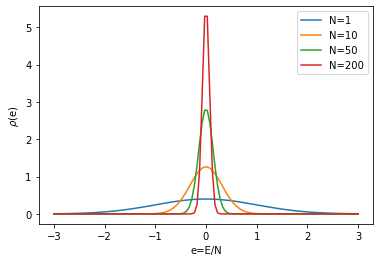
\includegraphics[width=0.7\textwidth]{Statistical mechanics/Images/E1B2D294-498C-45CC-AB94-2A59B549A443.png}
    \caption{As we increase N, the normal distribution becomes a sharp peak in the mean value (in this plot, it was used $\mu=0$ and $\sigma=1/\sqrt{N}$)}
\end{figure}


\paragraph*{Free energy and entropy}
As a last example, we are going to consider entropy. We can start by taking the definition of the entropy and then use the expression we found for the density function of the canonical ensemble:
\begin{equation*}
    \begin{split}
        S & = -k_B \int d\Gamma\, \rho\ln{\rho} \\
        & = -k_B \int d\Gamma\, \frac{e^{-\beta H}}{\mathcal{Z}}(-\beta H-\ln{\mathcal{Z}}) \\
        & = \left[\beta <H> +\ln{\mathcal{Z}}\right]k_B \\
    \end{split}
\end{equation*}
\begin{equation}
    S = \frac{<H>}{T}+k_B\ln{\mathcal{Z}}
\end{equation}
where we also used the expression we have already found on with $\beta$. Then we can define the \textit{Free energy} $F$ as:
\begin{equation}
    F= <H>-TS=-k_B T \ln{\mathcal{Z}}
\end{equation}
or alternatively as:
\begin{equation}
    e^{-\beta F}=\mathcal{Z}.
\end{equation}
For an ideal gas, we then get that:
\begin{equation}
    F=-k_B T \ln{\mathcal{Z}}=-k_B T \left[N\ln{V}+\frac{3N}{2}\ln{\left(\frac{2\pi m}{\beta} \right)}\right]
\end{equation}
and at this point we can also define the \textit{pressure} $P$ as:
\begin{equation}
    P=-\frac{\partial F}{\partial V}=\frac{k_B T}{V} N
\end{equation}
from which we can directly derive the \textit{equation of state of the ideal gas}:
\begin{equation}
    PV=N k_B T .
\end{equation}

As a final remark, we can use the expression we found for the partition function of an ideal gas in order to arrive at the expression for its entropy:
\begin{equation}
    S=\frac{3}{2}N k_B + N k_B \ln{\left[V\left(\frac{4\pi m E}{3N} \right)^{\frac{3}{2}} \right]}
\end{equation}
where we also used $\frac{1}{\beta}= k_B T= \frac{2E}{3N}$ by inverting the expression we previously found for the internal energy (here called $E$).

However, this expression can bring up a problem known as the \textit{Gibbs Paradox}, to which we only refer to the Huang-Kerson textbook (Statistical Mechanics, 2nd Edition, Chapter 6 paragraph 6). We just remark that the correct conclusion is based on the hypothesis that all the particles are indistinguishable: this is unjustified in Classical Mechanics and it is only explained in Quantum Mechanics. This hypothesis has as direct consequence that the correct expression of the partition function is given by dividing the previous one by $N!$ (a result also known as "correct Boltzmann counting") so that we end up with:
\begin{equation}
    \mathcal{Z}=\frac{V^N}{N!} \left(\frac{2\pi m}{\beta} \right)^{\frac{3N}{2}} \label{eq:zcannone}
\end{equation}
then the correct formulas for the entropy and the free energy are given in the thermodynamic limit, so that we can assume $\ln{N!}\approx N\ln{N}-N$; by repeating the calculation, we get:
\begin{equation}
    F=-k_B T \ln{\mathcal{Z}}=-k_B T \left[N\ln{V}-N\ln{N}+N+\frac{3N}{2}\ln{\left(\frac{2\pi m}{\beta} \right)}\right]
\end{equation}
and most importantly the correct, empirical expression for the entropy of the ideal gas:
\begin{equation}
\begin{split}
    S & =\frac{3}{2}N k_B + N k_B - N k_B\ln{N}+ N k_B \ln{\left[V\left(\frac{4\pi m E}{3N} \right)^{\frac{3}{2}} \right]} \\
    & =\frac{5}{2}N k_B+N k_B \ln{\left[\frac{V}{N}\left(\frac{4\pi m E}{3N} \right)^{\frac{3}{2}} \right]} \\
    & =\frac{5}{2}N k_B+N k_B \ln{\left[\frac{V(2\pi m k_B T)^{\frac{3}{2}}}{N} \right]}
\end{split}
\end{equation}
also known as the \textit{Sackur-Tetrode equation}. (As as side note: in this discussion we've never introduced the fact that we need in some cases a-dimensional quantities; this necessity implies the presence of a certain dimensional constant $h$, which is used in the Huang-Kerson textbook, corresponding to the Planck constant, which it was arbitrarily set equal to $1$ by Micheletti)